\documentclass[12pt]{article}

\usepackage{amsmath}
\usepackage{hyperref}
\usepackage{graphicx}

\begin{document}

\begin{titlepage}
    \centering
    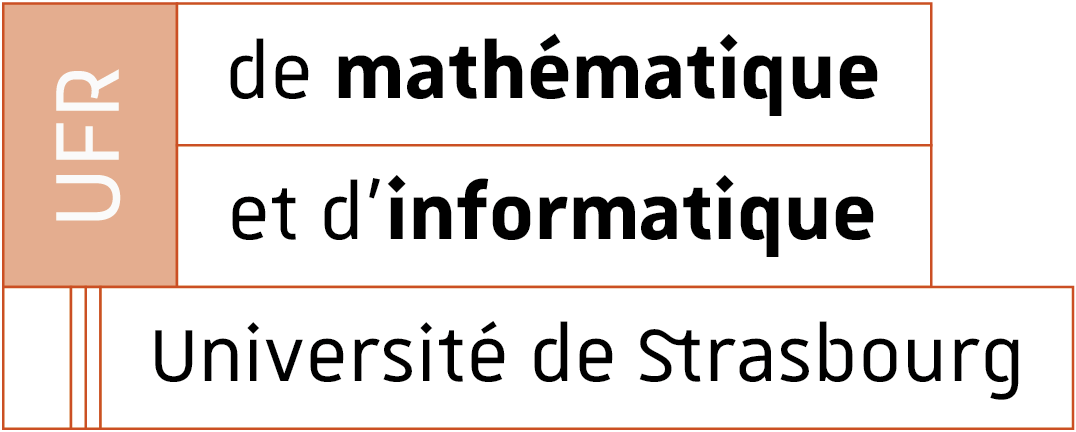
\includegraphics[width=0.5\textwidth]{images/logo_ufr.png}\par\vspace{1cm}
    \vspace{1.5cm}
    {\huge\bfseries ExaMA WP1 - Vegetation\par}
    \vspace{2cm}
    {\Large Giulio Carpi Lapi, Pierre-Antoine Senger\par}
    \vfill
    supervised by\par
    Pierre Alliez and Vincent Chabannes

    \vfill

% Bottom of the page
    {\large Date: \today\par}
\end{titlepage}

\tableofcontents
\newpage

\section{Abstract}
The abstract is a brief summary of your entire academic project report.
It typically provides an overview of the main objectives, methodology,
results, and conclusions of your research or project.
The purpose of the abstract is to give readers a quick understanding
of the key points of your work without having to read the entire document.
Key elements typically included in an abstract are:
Objective: A statement of the main purpose or objective of the project.
Methodology: A brief description of the methods or approaches
used to conduct the research or project.
Results: A summary of the main findings or outcomes of the project.
Conclusion: A brief statement of the implications or significance of the results.
The abstract is usually placed at the beginning of the report,
before the introduction, and should be concise, clear, and informative.
It helps readers decide whether they want to read the full report
by providing them with a preview of its content.

\section{Introduction}
A team of researchers is currently developing a tool for building
a 3D geometric model of an urban area (neighborhood, city, etc.).
This representation enables them to create
a thermal and energy simulation model.
For the moment, they can reconstruct the geometry of buildings and land
using information available in online databases such as OpenStreetMap, Mapbox, etc.
Vegetation (trees in particular) can have a significant impact on the model.
A tree can influence the temperature of the air, the ground, and the buildings.
It can also affect the energy consumption of buildings by providing shade or wind protection.
The goal of this project is to develop a method for adding vegetation to the 3D model.
The method should be able to create a realistic representation of the vegetation,
including the shape and size of the trees, their location, and their density.
The method should also be efficient and scalable to handle large urban areas.


\section{Literature Review}

\section{Methodology}

\section{Results}

\section{Conclusion}

\section{References}
\nocite{*}
\bibliographystyle{plain}
\bibliography{references}

\end{document}